

\newlength{\questlenght}
\settowidth{\questlenght}{\textbf{Question iii}\ \ }
\newlength{\textminusquest}
\setlength{\textminusquest}{\textwidth}
\addtolength{\textminusquest}{-\questlenght}
\newcommand{\ques}[2]{%
\noindent\textbf{Question #1}\hfill
\begin{minipage}[t]{\textminusquest}
    #2
\end{minipage}    
}


\chapter{Introduction}\label{chap:intro-english}


\begin{abstract}
abstract
\end{abstract}

\minitoc


\section{Motivation and positioning of the thesis}






\subsection{Probabilistic risk assessment studies}



\subsection{Uncertainty quantification in probabilistic risk assessment studies}



\subsection{The choice of the prior in Bayesian studies}

\subsection{Motivating prior elicitation research for SPRA studies}



\section{Outline of the manuscript and contributions}

\subsection{Problems statement and organization of the thesis}



\subsection{List of contributions}













\chapter{Introduction en français}\label{chap:intro-french}

\renewcommand{\chaptername}{Chapitre}
\renewcommand{\partname}{Partie}


\begin{abstract}[Résumé]
    Ce chapitre ne diffère du \hyperref[chap:intro-english]{chapitre 1} que par sa rédaction en langue française.
    Dans ce chapitre, nous introduisons et motivons les travaux de recherche qui ont été conduit au court de cette thèse. Les travaux sont motivés
    principalement par le besoin d'évolution des méthodes d'études sismiques probabilistes de sûreté, mais aussi par le manque de réponse qu'apporte l'état-de-l'art à la question du choix du prior en inférence bayésienne.
    Ces problématiques sont détaillées et
    les travaux sont alors introduits comme s'inscrivant dans celles-ci, le tout donnant lieu à une organisation consistante du manuscrit.
    %en introduisant à la fois leur inscription dans le cadre des études sismiques probabilistes de sûreté et dans le
    %
    %D'une part, nous introduisons le cadre des études sismiques probabilistes de dûreté, et 
    % Dans ce chapitre, nous mettons en lumière les différentes problématiques, à la fois issue de qui motivent 
    % Dans ce chapitre, nous introduisons les différents contextes qui motivent l'existence de cette thèse. D
\end{abstract}

\minitoc

\section{Motivation et positionnement de la thèse}

\subsection{Etudes probabilistes de sureté}
%

\subsubsection{Historique}

Les études probabilistes de sureté (EPS) désignent un ensemble de méthodes d'analyses techniques qui permettent de quantifier un risque encourut par une installation lorsqu'elle est sujette à un évenement. L'évenement peut être d'origine naturelle comme artificielle, il peut être de provenance interne comme externe ; il peut s'agir d'un séisme, d'une inondation, d'une combinaison de défaillances internes, entre autres.  % (qui peut être d'origine naturelle comme artificielle, qui peut être interne comme externe). 

Faisant suite au premières recommandations de F. R. Farmer (expert sûreté à la UK atomic authority) dans les années 1960 pour la fiabilité des installations nucléaires,
ces méthodes ont pour caractéristique commune l'introduction de la notion d'incertitude dans la qualification de l'évenement, ses phénomènes et ses caractéristiques (on parle alors d'aléa).
%
%Elles ont été introduites par F. R. Farmer dans les années 1960 [], qui plébiscitait cette idée d'étudier la fiabilité des installations nucléaires en prenant en compte l'aspect probabiliste et incertain des évenements auqelles elle est sujette.
%
Leur cadre et leur concept ont été rapidement adoptés et développés aux Etats-Unis (cf. le raport de la Nuclear Regulatory Commission, \cite{nrc_pra_1983}). En particulier, de nombreuses études sont venues dès 1968 (\cite{cornell_engineering_1968}) 
y inscrire les analyses de fiabilité parasismique, définissant alors le cadre des études simsiques probabilistes de sureté (SPRA en anglais). %, en particulier en ce qui concerne le cadre de la fiabilité parasismque.



Le séisme représente en effet un facteur de risque remarquable des études de sureté.
Premièrement, bien que communément caractérisé par sa magnitude et sa distance à la source, son signal est bien plus riche qu'une fonction bivariée et deux séismes de même magnitue et de même source peuvent avoir des caractéristiques (et des conséquences) significativement différentes.
Deuxèmement, puisqu'il touche à la fois tous les élements aussi bien externes qu'internes à l'installation, il est la potentielle source de conséquences lourdes sur les équipements et structures.
%voir de réactions en chaîne 
%qui atteindraient le ``noyau dur'' de l'installation (défini comme un ensemble d'élements critiques à l'installation). %, impliquant ainsi un coût élevé.
Le coût potentiel des conséquences d'un aléa sismique peut alors être élevé et critique dans le contexte nucléaire, ce qui fait en fait un évenement d'intérêt majeur et décisif même dans les zones géographiques où il est rare.


%La prise en compte du séisme comme un aléa s'est confronté à la

Aujourd'hui, la prise en compte de l'aléa sismique sous le cadre des études probabilistes de sûreté est une recommandation internationale dans le contexte de l'industrie nucléaire. Leur cadre d'application dans l'industrie nucléaire française est précisé par l'autorité de sureté nucléaire et de radioprotection (ASNR)\footnote{Anciennement ASN: l'autorité de sûreté nuclaire (ASN), a été unifiée avec l'institut de radiprotection et de sûreté nucléarie (IRSN) le 1\textsuperscript{er} janvier 2025.} dans la règle fondamentale de sûreté (\cite{asn_regle_2002}).









\subsubsection{L'évolution des EPS en France, au CEA, et dans cette thèse}



%Le rôle des études de sûreté d'une manière générale est de produire une quantification du risque d'une installation, d'une marge de fiabilité, et de démontrer son repsect d'un seuil défini par une autorité de régulation.
% Deux visions s'oppose relativement au sujet de l'avolution des méthodes et des conaissances relatives aux études de sûreté.
%Lors de la mise en place de de seuil et de la règle, plusieur point de vue, motivés par plusieurs intérêts peuvent alors se heurter. Il y a d'une part les exploitants, pour qui la notion de robustesse perdure d'elle même, les marges prises sont là pour tenir compte du manque de conaissances, et il y a ceux pour lesquels la robustess est sans cesse remise en question par les avancées des méthodes et des connaissances (\cite{roger_seisme_2020}).



%L'évolutions des méthodes et des conaissances relatives à la sûreté de 
L'évolution des méthodes et des conaissances relatives à la sûerté des installations nucléaires se fait de manière parallèle à l'évolution de la règle et de la norme imposées à celles-ci. 
Sur le sujet de l'aléa sismique, le rapport à l'évolution de la règle et de la méthode (et donc des EPS) oppose différents points de vue, princpalement entre le principal exploitant (EDF) et les experts de l'autorité de sûreté (anciennement l'IRSN, maintenant unifié avec l'autorité de sûreté nucléaire devenue l'ASNR). 
Pour le premier, la robustesse de l'installation n'est normalement pas remise en question par l'avancée des conaissances et des méthodes puisque l’incertitude sur celles-ci fait parti des marges prises en comptes à la construction de l'équipement et calculées pour. Le second pense au contraire que la robustesse est une question perpétuelle et que la marge n’est pas pas faite pour être mordue au fil des connaissances qui s’ajoutent (\cite{roger_seisme_2020}). 
% L'évolution des méthodes EPS reste un champ de voies ouverte, pour lequel les approches s'opposent fondamentalement.
%Il est complxe de définir une voie d'évolution des EPS, et il n'y a pas de vision qui fait l'unanimté
L'ASNR se place alors en arbitre dans ce dialogue, entre autre elle définit le ``séisme majoré de sécurité''\footnote{Aujourd'hui plutôt appelé ``séisme noyau dur''.} (il s'agit d'une majoration du spectre du ``séisme maximal historiquement vraisemblable''\footnote{Aujourd'hui plutôt appelé ``séisme de dimensionnement''.}) qui sert de marge de référence dans la démonstration de robustesse parasismique d'un équipement. % la marge de fiablité et séisme maximal à prendre en compte. %En ce qui concerne l'aléa sismique, le dialogue 
%
%Un tel dialogue n'est pas propre à la France, et 


Cet arbitrage est donc à la fois sensible et critique.
L'incident survenu en 2011 à la centrale nucléaire de Fukushima-Daiichi le démontre. L'aléa sismique (qui est la cause du tsunami) de référence
%fixé par le concensus des experts japonais
a été sous-évalué par le consensus des experts japonais, et c'est cette sous-évaluation qui est au final la cause de l'incident (cf. le rapport de l'agence internationale de l'énergie atomique, \cite{iaea_fukushima_2015}).
%En 2011, a eu lieu un incident 
Suite à cet évenement, l'ASNR a pris la décision de majorer d'un facteur 1.5 le séisme majoré de sécurité en France, imposant une démonstration amplifiée de la robustesse des différentes installations par leur exploitant.



%En 2011, à la suite de l'incident à la centrale de Fukushima suite au séisme survenu au large des côtes japonaises, ce dialogue s'est conclut par une imposition de la part de l'autorité de sûreté d'une majoration d'un facteur de 1.5 de ce séisme majoré de sécurité en France. % de la marge de fiabilité sismique des équipements nucléaires en France. 

%Devant le coût induit par 

%Cette différence démontre de la complexité du sujet






% Le séisme ne fait pas exception
% la place des EPS simsique dans cette différence de vision est très marquée puisque l'aléa du séisme reste une quesiton ouverte en soi, la moindre différence de choix de séisme maximim possible peut donner lieu à une ampleur de changement d'un coût très élevé pour l'exploitant



%Les études probabilistes de sureté ont été adoptées progressivement en France 


%En France, l'industrie nucléaire est réduite à un nombre restreint d'acteurs, exploitants, experts indépendants, et autorité.

% Ambivalence de la robustesse, deux notions 
% deux visions
% Le CEA, à la fois exploitatn et expert

La place du CEA est ambivalente dans l'échiquier nucléaire français.
D'une part, il est exploitant d'installations nucléaires de recherche 
et joue alors son propre rôle quant à la démonstration de robustesse de ses équipements.
Aussi,
%, et ausi %titulaire d'une mission d'expertise de sûreté.
il participe à l'expertise conjointe des expertises de sûreté relatives au parc nucléaire civil exploité par EDF. 
%Le CEA joue son propre rôle dans l'évolution de la démonstration de la robustesse de ses propres equipements et installations. 
La recherche et l'expertise sur les causes de l'aléa sismique % études simqiques de sûreté au CEA 
se fait au CEA au laboratoire EMSI, qui dispose d'une plateforme experimentale (Tamaris) qui permet de procéder à divers tests mécaniques sur des équipements sous séismes. 
%Le laboratoire d'etudes mécaniques et sismiques (EMSI) s'inscrit pleinenemnt dans cette ambivalence. Propriétaire de la plateforme d'expérimentation sismique Tamaris, le labortoire se place souvent au centre des études de fiabilité sismique et du dialogue entre EDF et les experts de l'ASNR.
L'approfondisemnt des méthodes des études sismiques probabilistes de sûreté est un enjeux du CEA qui s'inscrit dans ce laboratoire. Le CEA étant responsable devant les autorités de sûrété de ses installations, il cherche %alors 
à développer des méthodes toujours rigoureuses devant leur vieillissement. %de ces installations et de leurs équipements.



% Le rôle du CEA est ambivalent dans cete equation, à la fois exploitant instut de recherche.
% Le CEA joue son propre rôle dans l'évolutions de la démonstration de robstesse de ses propres installations. Aussi il participe à l'expertise conjointe de méthodes d'EPS avec EDF.


% Le CEA est lui même exploitant, d'unstallations de recherche.
% Il a 

% L'evolutio des EPS y est toujours un enjeux pour être capable de produire une étude plus efficace, et des résultats plus convaincants aurpès des autorités.
% Le CEA est responsable auprès des autorités concernant ses installations et cherche à développer des méthodes toujours rigoureuses devant le vieillissemnt des installations

% Sur le sujet de l'aléa sismique, la démonstration de robustesse reste complexe vis à vis de la complexité de l'aléa lui-même, et de sa fréquence.
% Les EPS sont en constantes ré-évaluation à la demande des autorités de sûreté sur cette aspect, principalement depuis l'accident sur la centrale de Fukushima en 2011. %%% Peut etre mettre ca plus haut

% Au CEA, la recherche sur les études sismiques probabilistes de sûerté est portée par le laboratoire EMSI, qui dispose d'une plateforme experimentale (Tamaris) qui permet de procéeder à divers tests mécaniques sur des équipements sous séismes. 

Cette thèse s'inscrit dans la démarche d'évolution du SPRA et de démonstration de sûreté. Financée par le CEA dans le cadre d'un contrat de formation par la recherche, elle a pour objectif d'étoffer l'état de l'art en terme d'estimation de fragilité sismique des equipements et des installations.
L'objectif est de développer des méthodes qui doivent le mieux possible être (i) efficaces devant la complexité des objets étudiés et de la définition de l'aléa, (ii) être robustes dans le temps et devant une potentielle réévaluation des critères de sûreté, et (iii) être transparentes et auditable par les autorités de sûreté.

%lieu à des méthodes qui savent être efficace devant la complexité technique représentée efficaces devant la c

%en cherchant un cadre plus robuste, plus efficace.
%%%% Principalement en appuyant l'étude bayésienne de celles-ci.




\subsection{La quantification d'incertitudes dans les études probabilistes de sûreté} % la quantification d'incertitutde dans les EPS


\subsubsection{Principe et étapes de la quantification d'incertitudes}

%Le cadre des EPS regroupe un certains nmb
%Différents outils mathématiques sont employés dans le cadre des EPS et composent

Les études probabilistes de sûreté %et plus généralement les études probabilistes de fiabilité, de robustesse, et de  %les procédés de génie probabiliste d'études de fiabilité, de robustesse, et de 
s'appuient sur la 
prise en compte et la quantification des incertitudes qui apparaissent dans le procédé d'évaluation d'un risque au sein d'un système physique.
%lors de l'évaluation d'une quantité décrivant un risque. %d'un 
%
La quantification d'incertitudes représente en fait une démarche qui consiste à modéliser et analyser méthodiquement l'incertitude, sa source, et sa propagation au sein de la modélisation du système physique étudié. %étudié. %système phyisique?
Elle se construit alors à l'intéraction de la physique, de l'ingéniérie et des mathématiques appliquées, et s'érige même comme une branche des statistiques à part entière.

Elle concentre son étude sur 3 éléments qui décrivent l'intéraction entre le système physique et l'aléa : des paramètres d'entrée $\mbf X$, une réponse physique du système $ Y$, et une modélisation de celle-ci selon : $ Y=\cM(\mbf X)$. % ($\cM$ peut-être définit comme la ).
Cette fonction $\cM$ est liée à la modélisation, souvent complexe, du système et de ses proporiétés physiques (il peut s'agir de la résolution d'équations physiques, de simulation numériques, ou même du résultat d'une expérience mécanique).
%L'objet de la quantification d'incertitude est alors d'évaluer une quantité d'intérêt qui dépend de $\mbf Y$ : comme une variance, une probabilité de défaillance, etc ; plus généralement une quantité de la forme $\EE\,\phi(\mbf Y)$.
%
La démarche générale de la quantification d'incertitudes est souvent décrite au travers de différentes étapes clées (voir par ex. \cite{sudret_uncertainty_2007, iooss_contributions_2009}), à savoir : %au sein desquelles on distingue particulièrement l'étape d'identification des sources d'incertitudes.
%qu'on peutt principalement résumé 
%
\begin{enumerate}
    \item L'identification des sources incertitudes : 
        il est usuel de classifier les incertitudes selon deux grandes catégories. D'une part les incertitudes irréductibles, qui proviennent du hasard ``naturel'' embarqué dans l'aléa et le système physique. D'autre part, les incertitudes épistemiques, qui existent par manque d'information, et qui sont alors considérées comme réductibles en opposition aux précédentes (\cite{hullermeier_aleatoric_2019}). Il s'en suit une modélisation probabiliste de l'entrée $\mbf X$. 
    \item La propagation des incertitudes : cette étape correspondant à l'approximation de la distribution du modèle $\cM(\mbf X)$, et de l'évaluation d'une quantité d'intérêt qui dépend de celle-ci : comme une variance, une probabilité de défaillance, etc ; plus généralement une quantité de la forme $\EE\,\phi( Y)$.
%     et de celle de la quantité d'intérêt $\phi(\mbf Y)$. %De nombreuses méthodes mathématiques viennent en appui à cette étape, et sont évoquées plus bas.
    \item L'analyse de sensibilité : son rôle est de comprendre avec plus de recul la manière dont l'incertitude se propage dans un système, en identifiant l'impact d'un ou de plusieurs des paramètres d'entrées sur la sortie $ Y$ (\cite{iooss_review_2015}).
    %L'analyse de sensibilité se construit depuis les premier travaux de Sobol' (\cite{sobol_sensitivity_1993})
    %, lorsque les entrées sont multivariées ($X=(X_1,\dots,X_p)$), quelles sont celles  
\end{enumerate}


\subsubsection{Des outils mathématiques en quantification d'incertitutdes}

%L'étape 1 sus-mentionnée s'ajoute à la modélisation du  modélisation
%Les étapes 2 et 3 ci-dessus mentionnées 
De nombreux outils mathématiques viennent appuyer les etapes sus-mentionnées. Bien que ce manuscrit n'a pas pour but d'en décrire un pannel exhaustif, ci-dessous sont listés quelques exemples qui reviennent dans les travaux de cette thèse.
%en voici quelques uns qui sont omniprésents dans le domaine

\begin{itemize}
    \item La métamodélisation %, %le plus souvent par processus gaussien (appellé aussi krigeage), ou par polynomes du chaos, 
    permet de contrevenir la complexité d'évaluation du modèle $\cM$, en construisant un métamodèle $\tilde\cM$, entraîné à partir d'une base de données d'observations $(\mbf x_1, y_1),\dots,(\mbf x_k,y_k)$. Le méta-modèle se veut par principe plus simple à évaluer que le modèle réel. 
    Rien ne limite sa définiton explicitement qui peut aller d'un simple modèle paramétrique à la sortie d'un réseau de neurones ``boite noire'' ; parmi les plus commun on peut évoquer la méta-modélisation par processus gaussien (ou krigeage) et par polynômes du chaos. %Dans le cadre d'études de sûreté, on citera par exemple \cite{}
    %
    \item Les indices globaux de sensibilité s'inscrive pleinement dans l'étape d'analyse de sensibilité du système.
    % 
    Ils consistuent depuis les premiers travaux de \citet{sobol_sensitivity_1993} des outils essentiels pour mesurer statistiquement comment $ Y$ est impactée par un ou plusieurs des $X_i$ (où $(X_1,\dots,X_p)=\mbf X$). Dans ce cadre, l'impact, noté $S_i$, de l'entrée $X_i$ sur $ Y$ s'exprime comme une divergence moyenne entre la distribution $\PP_{ Y}$ de $ Y$ et sa distribution conditionalement à $\mbf X$, $\PP_{Y|\mbf X}$ \citep{da_veiga_global_2015} : 
        \begin{equation}
            S_i = \EE_{X_i}[D(\PP_{ Y}||\PP_{Y|X_i})],
        \end{equation}
    où $D$ est une mesure de dissimilarité entre deux mesures de probabilité.
    Le choix de $D$ est alors décisif dans l'étude de $S_i$. %, qui revient à une étude de divergence entre deux mesures de probabilité. 
    On peut noter, par example, que choisir $D$ définie par $D(P||Q) = \|\EE_{X\sim P}X-\EE_{X\sim Q}X\|^2$ revient à étudier un indice de Sobol' du premier ordre.
    Le choix de $D$ peut être motivé par divers intérêts, par exemple, celui de discriminer  l'indépendance entre $X_i$ et $ Y$. Le point suivant détail un large pannel de choix possibles pour $D$.

    \item La théorie de l'information est au centre de la comparaison de mesures de probabilité et donc de la quantification d'incertitudes. Par essence, les manières de comparer la façon qu'ont deux mesures de probabilité de  distribuer l'information dans un espace sont vastes. 
    Dans la définition de $S_i$ plus haut, le choix de $D$ (et donc le choix de définition de $S_i$) relève de la théorie de l'information.
    
    
    % , puisque deux distributions difères par la manière dont elles 
    Un choix alors commun, perçu comme une extention de l'entropy de Shanon, est celui des $f$-divergences de \citet{csiszar_information-type_1967}. On peut noter qu'elles sont employées dans des domaines variés, au delà de l'analyse de sensibilité, tel que l'inférence variationnelle (\cite{minka_divergence_2005,bach_sum--squares_2023}), le design de méta-modèles (\cite{nguyen_surrogate_2009}), l'apprentissage PAC-bayésien (\cite{picard-weibel_change_2022}).
    Lorsque $f$ est convexe que $f(1)=0$, elle sont définies selon :
        \begin{equation}\label{eq:intro-fdiv-french}
            D_f(P||Q) = \int_\cX f\left( \frac{p(x)}{q(x)} \right) q(x)d\mu(x),
        \end{equation}
    en notant $p$, $q$ des densités associées à $P$ et à $Q$ par raport à une mesure commune $\mu$ sur leur ensemble de définition $\cX$.     
    Les $f$-divergences réduisent le choix de $D$ à celui de $f$, les plus communément employées étant les $\delta$-divergences (\cite{zhu_information_1995}) définies en fixant $f=f_\delta$ où
        \begin{equation}
            f_\delta(x) = \left\lbrace\begin{array}{l l} \frac{x^\delta-\delta t-(1-\delta)}{\delta(\delta-1)} & \text{si\ }\delta\not\in\{0,1\},\\ 
                t\log t-t+1  & \text{si\ }\delta=1, \\
                -\log t +t -1 & \text{si\ }\delta=0.
            \end{array}\right. 
        \end{equation}    
    Il est remarquable que la peut-être plus connue des mesure de dissimilarité (la divergence de Kullback-Leibler) peut être vu comme un cas particulier des $\delta$-divergences. En effet, rappelons que la divergence de Kullback-Leibler, notée $\text{KL}$, est définie par 
        \begin{equation}
            \text{KL}(Q||P) = \int_\cX\log\left(\frac{q(x)}{p(x)}\right)q(x)d\mu(x)
        \end{equation}
        (en adoptant les même notations qu'en équation \eqref{eq:intro-fdiv-french}), si bien que 
        \begin{equation}
            D_{f_\delta}(P||Q) = \text{KL}(P||Q)\ \text{si\ }\delta=1,\quad D_{f_\delta}(P||Q) = \text{KL}(Q||P)\ \text{si\ }\delta=0.
        \end{equation}

    Bien sûr, il existe aussi de nombreuses mesures de dissimilarité qui ne sont pas des $f$-divergences, à ce titre, les indices de Sobol' du premier ordre évoqués plus haut font offices d'exemple. Un autre exemple notable présenté ici est celui des normes maximales de discrépences (MMD). Soient $P$, $Q$ deux mesures de probabilité définies sur un ensemble $\cX$, et soit $\cH$ un espace de Hilbert à noyau reproduisant (RKHS) sur $\cX$,  dont le noyau reproduisant est noté $k:\cX\times\cX\to\CC$. %On peut définir les imbrications moyennes  \cite{gretton_kernel_2012}
    On définit la MMD (\cite{gretton_kernel_2012}) par
        \begin{equation}
            \text{MMD}(\cH;\,P||Q) = \sup_{\substack{f\in\cH\\ \|f\|_\cH\leq1}} |\EE_{X\sim P}f(x) - \EE_{X\sim Q}f(X)|,
        \end{equation}
    ou, dans une forme plus simple :
        \begin{equation}
            \text{MMD}^2(\cH;\,P||Q) = \EE_{X,X'\sim P\otimes P}[k(X,X')] + \EE_{Y,Y'\sim Q\otimes Q}[k(Y,Y')] - 2\EE_{X,Y\sim P\otimes Q}[k(X,Y)].
        \end{equation}
        %
    \item L'analyse bayésienne est outil incontournable de la quantification d'incertitude, puisqu'elle a pour principe fondamental d'introduire une forme d'incertitude dans un ou plusieurs des paramètres du modèle étudié. 
    L'incertitude incorporée par le cadre bayésien peut prendre diverse forme, et se traduit au travers de la définiton de l'\emph{a priori}. 
    La propagation d'incertitudes au travers de ce canevas se quantifie en calculant l'\emph{a posteriori}, à partir d'observations statistiques $(\mbf x_1,y_1),\dots,(\mbf x_k, y_k)$.
    La définition de l'\emph{a priori} est critique, elle prend place dans l'étape d'identification des incertitudes, et se révèle impactante sur l'\emph{a posteriori}, et donc, dans un contexte d'étude probabiliste de sûreté, sur le risque.
    
    Puisque ce dernier outil, qui est en fait un paradigme à lui tout seul, est au centre de cette thèse, la section qui suit lui est pleinement dévoué.
\end{itemize}
















\subsection{Le choix du prior dans les études Bayésiennes}

%L'inférence Bayésienne s'inscrit dans le domaine de l'inféérence statistique.
% ici paradigmes freq bayes et intervalles cred conf


L'analyse bayésienne est une théorie des statistiques qui se construit selon une interprétation des probabilités qui sont vues comme des degrés de plausibilité des évenements, on parle généralement de ``crédibilité''. 
%Comme toute théorie statistique =
Comme toute étude statistique, elle cherche à faire le lien entre des observations statistiques et leur distribution probabiliste. %, avec comme particul identifier la distribution de données observée.
Elle s'appuie sur le théorème de Bayes, en considérant l'inconnu qui permet de définir la distribution des données comme étant aléatoire. Les observations statistiques informent alors la distribution de cette inconnue, ce qui met  à jour le degré de crédibilité attribué à une distribution que suivraient les données par rapport à une autre.


Le raisonemement contraire, dit fréquentiste, considère la probabilité comme une fréquence d'occurence observable au prix de reproduire l'expérience. Sous ce paradigme, l'inconnue existe, 
et les fréquences données par la répétition de l'expérience sont plus probables selon que l'on considère certaines valeurs de l'inconnue plutôt que d'autres, on parle généralement de ``confiance''.


Au final, il est important de noter que ces deux raisonement se complètent, voir parfois se confondent suivant les cas, et ils sont loin d'être antinomiques. Dans un contexte pratique, le cas d'étude et ses spécificités peuvent néanmoins orienter le choix de favoriser l'un par rapport à l'autre.

%et c'est alors l'aléatoire observé lors de cette répétition qui traduit la confiance en une distribution pluôt qu'en une autre %de l'observation aléatoire qui définit

Dans cette thèse, on se concentre sur l'analyse bayésienne dans le cadre de l'inférence statistique. Dans ce contexte, une variable d'intérêt $Y\in\cY$ est modélisée selon une distribution paramétrique $\PP_{Y|\theta}$, $\theta\in\Theta$ étant l'inconnue, alors considérée comme étant une variable aléatoire dans le canevas Bayésien.
En toute logique, $\theta$ admet une distribution, que l'on appelle le \textbf{prior}.
Lorsque des réalisations de $Y$ successives et indépendantes conditionnelement à $\theta$ sont observées, le \textbf{posterior} se définit comme la distribution de $\theta$ condtionnelement à ces observations. Une région de crédibilité à un niveau $r$ se définit comme une région de $\Theta$ dont la probabilité selon le posterior est au moins égale à $r$.
On notera que dans ce contexte, divers résultats lient les approches bayésienne et fréquentiste d'estimation de $\theta$. Le théorème de Berstein Von-Mises (voir par ex. \cite{van_der_vaart_asymptotic_1992}) en est un exemple.


Notons $\mbf y = (y_1,\dots,y_k)$ les valeurs observées de $k$ réalisations de $Y$. En supposant que tous ces objets existent et sont bien définis, notons $\pi$ la densité du prior (selon une mesure $\nu$), $\ell(\cdot|\theta)$ les densités de $\PP_{Y|\theta}$ (selon une mesure $\mu$) et  $\ell_k(\mbf y|\theta)=\prod_{i=1}^k\ell(y_i|\theta)$, appelée la vraisemblance du modèle. Alors avec ces notations le théorème de Bayes définit la densité du posterior (par rapport à $\nu$) selon :
    \begin{equation}
        p(\theta|\mbf y) = \frac{\ell_k(\mbf y|\theta)\pi(\theta)}{\int_{\Theta}\ell_k(\mbf y|\theta)\pi(\theta)d\nu(\theta)  }.
    \end{equation}
Cette formule fait le lien entre le prior, le modèle (représenté par la vraisemblance), les données, et le posterior qui traduit la prédiction crédible. Elle permet de schématiser le canevas bayésien comme une chaine de transmission d'information vers l'\emph{a posteriori}, depuis deux sources : le ``réel'' (les observations) et l'\emph{a priori}. Ce schéma est celui présenté ci-dessous.
    \begin{figure}[h]
        \centering
        \begin{tikzpicture}

            \draw[-{Latex[length=1.5mm]}] (-0.4, 0) -- (.5, 0); % english (0, 0) -- (.9, 0); 
            \draw (-0.4, 0) node[left] {Base de données $\mbf y=(y_i)_{i=1}^k\in\cY^k$}; %english (0,0)
             
            \draw (2.4, 0) node {vraisemblance ${\ell_k(\mbf y|\theta)}$}; %englih (2.5,0)
            
            \draw[-{Latex[length=1.5mm]}] (-0.4, -0.6) -- (0.5, -0.6); % english (0, -0.6) -- (0.9, -0.6); 
            \draw (-0.4,-0.6) node[left] {Paramètre $\theta\in\Theta$}; %english (0,-0.6)
            
            \draw (2.4,-0.6) node {prior $\pi(\theta)$}; % english (2.5,-0.6)

            \draw [-] plot [smooth] coordinates {(4.3,0) (4.6,-0.03) (5.05,-0.27) (5.5,-0.3)};
            \draw [-{Latex[length=1.5mm]}] plot [smooth] coordinates {(4.3,-0.6) (4.6,-0.57) (5.05,-0.33) (5.5,-0.3)};

            \draw (5.7,-0.3) node[right] {posterior $p(\theta|\mbf y)\propto{\ell_k(\mbf y|\theta)}{\pi(\theta)}$};
            
        \end{tikzpicture}
    \end{figure}

%D'une certaine manière

Si l'information issue des données ne pose normalement pas question, c'est l'information \emph{a priori} qui concentre l'attention. Par essence, elle est la source de l'incertitude dans le résultat,  sa construction doit se faire de manière attentive lors de l'étape de modélisation et ne peut être arbitraire. 
%On peut noter également que l'information issue des données passe aussi bien au travers du modèle, tel que la vraisemblance le décrit. Cette modélisation qui est alors au centre 
%Différents auteurs placent aujourd'hui la sélection, la validation et la mise à jour du modèle au centre des études bayésienne, définissant cette démarche comme le worflow bayésien \cite{gelman_bayesian_2020}.
Cependant, la formulation bayésienne lui attribue un impact significatif sur le postrior, particulièrement dans des cas où la taille de la base de données est limitée. Une illustration de ce phénomène est proposée en figure~\ref{fig:intro-differentsposteriors}, où différents priors, en apparence proche, donnent lieu à des posteriors très différents, à partir des même observations.
Bien sûr, le diable est dans les détails, et ici, ce sont les queues de distributions des priors, peu discernable sur l'illustration, qui produisent cette différence. Malgré tout cet exemple questionne, et à juste titre, sur le choix du prior.

\begin{figure}[h]
    \centering
    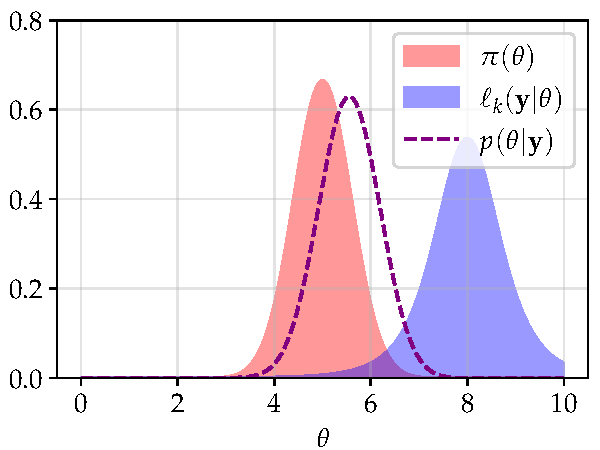
\includegraphics[width=5cm]{figures/intro/posterior1.pdf}
    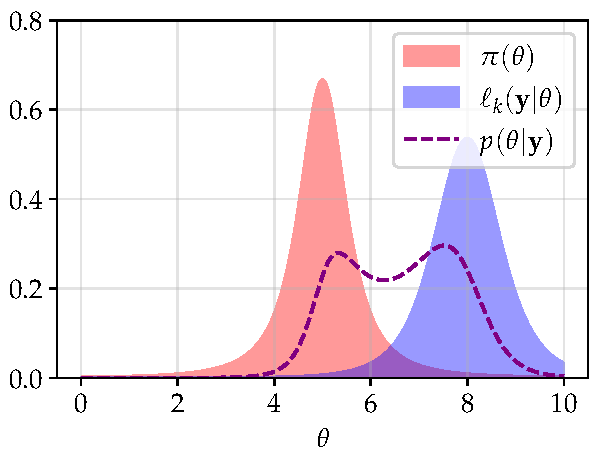
\includegraphics[width=5cm]{figures/intro/posterior2.pdf}
    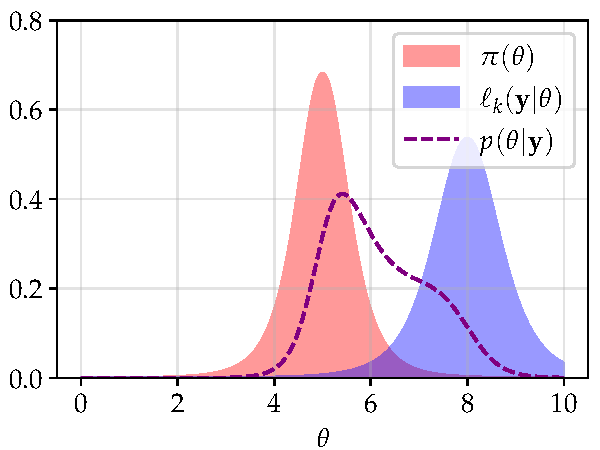
\includegraphics[width=5cm]{figures/intro/posterior3.pdf}   
    \caption{Différents calculs de postériors (en pointillé) à partir d'une même vraisemblance (bleu) mais de différents priors (rouge).%De gauche à droite le prior est : une gaussienne $\cN(5,)}
    }
    \label{fig:intro-differentsposteriors}
\end{figure}


%On peut déduire d'un tel exemple que les queue de distribution repésente une information décisive au sein d'un prior. Cela illustre 

La question de la construction du prior reste une question ouverte dans la littérature. %tout le worflow bayésien \citep{gelman_bayesian_2020}, elle oppose souvent deux répons%es possibles
%Elle oppose souvent deux axes de refléxions : la définiton de p
Pour certains, elle est l'opportunité d'ajouter de l'information provenant d'une source extérieure, il peut s'agir d'un jugement d'expert, de données historiques, ou de conaissances sur certaines propriétés attendues du résultats. Leurs priors sont plutôt qualifiés d'informatifs.
Pour d'autres, elle est au contraire le moyen d'introduire une incertitude dans le modèle, l'\emph{a priori} est alors dans un tel cas une absence de conaissance, qui vient laisser l'information provenir essentiellement des données. Ces derniers ont confiance en la modélisation de la vraisemblance, et leur prior sera qualifié de non-informatif.


On comprend au travers de ces paragraphes introductifs que cette question est insoluble : il ne peut pas exister de méthode unanime de sélection de prior. Elle illustre même l'un des ``trous'' du worflow bayésien selon \citet{gelman_holes_2020} : les priors trop informés ne permettent pas d'avoir confiance en le moindre résultat tandis que les priors trop peu informés %n'exerguent que trop peu d'estimation crédible.
donnent lieu a des zones de crédibilité parfois trop larges et inutilisable.
%Il ne s'agit pas de décrédibiliser le bayésien 
Ce n'est pas pour autant que l'approche bayésienne perd son intérêt et cette section n'est pas vouée à discréditer la démarche, la suite du manuscrit le prouvera. %Comme toute méthode elle doit être construite 
Mais elle doit laisser celui ou celle qui l'emploi conscient ou consciente des impactes et des limites de ses choix. Le choix d'un prior est aussi critique que le choix du modèle lui-même.








%Lorsque l'on observe plusieurs réalisations de $Y$ sont observées : $(Y_1,\dots,Y_k)$






\subsection{Ce qui motive la recherche sur l'elicitation de priors pour les études sismiques probabilistes de sûreté}

L'analyse bayésienne a gagné en popularité dans de nombreux domaines, y compris dans des études de fiabilité ou de sûreté. 
En effet, elle est plébiscitée pour sa capacité (i) à introduire et propager une incertitude dans un problème d'inférence, et (ii) à être plus régulière que beaucoup de métodes fréquentistes, en particulier lorsque le nombre de données observées est limité.

Le cadre de l'inférence bayésienne s'introduit en effet bien dans la démarche de quantification d'incertitudes. 
L'identification des incertitudes sur l'entrée $\mbf X$ ou sur le modèle même $\cM$ (ou bien s'il y a lieu le méta-modèle) peut se faire au travers d'une paramétrisation de celles-ci, en donnant lieu à une distribution paramétrique de $Y$ : $\PP_{Y|\mbf X,\theta}$.
La variable $\theta$, aléatoire sous le paradigme bayésien, peut alors représenter diverses sources d'incertitudes, de différentes natures selon les cas \citep{bousquet_contributions_2024}. Cette approche a été employée à pléthore dans divers types de modèles, on peut citer par exemple le cas de processus gaussiens (par ex. \cite{gu_parallel_2016}) ou des réseaux de neurones \citep{arbel_bayes_2023}. 



Parfois, certaines études adoptent la démarche pour la possibilité qu'elle offre d'introduire un jugement  ou une conaissance \emph{a priori}.
C'est pourtant ce même point qui fait aussi débat puisqu'il est la potentielle source d'une subjectivité difficile à justifier.
Dans le cadre des études sismiques probabilistes de sûreté en industrie nucléaire, la démonstration de robustesse est centrale. Les cas d'études y étant souvent très complexes, on trouvera alors parfois autant de priors qu'il y a d'experts en suivant cette démarche.
De tels cas caricaturaux mettent en péril l'auditabilité de la moindre région de crédibilité \emph{a posteriori}.

%De fait, il est essentiel de se chercher à se prévaloir 
%De telles études, compatibles et 
%nécessite l'apport d'un cadre méthodique et rigoureux de 

On comprend en fait que dans une étude de sûreté qui se veut auditable, une ``bonne'' région de credibilité sur un paramètre estimé n'est pas une région nécessairement étroite, même si elle suggère que la sûreté est satisfaite. A l'inverse, une région trop large n'est pas pour autant ``bonne'' car elle ne permet pas de démontrer la robustesse attendue de l'equipement. L'équilibre est complexe, et le ``bon'' prior est celui qui, bien que démontrant au mieux la capacité où l'incapacité de l'equipement à résister à l'aléa, produit un résultat inspirant confiance. %Il doit être assuré qu'il est affranchi de l'introduction d

Toutes ces réflexions mettent en lumières l'intérêt d'une construction méthodique du prior dans le cadre des études sismiques probabilistes de sûreté, au travers d'un cadre rigoureux qui évite l'introduction de la moindre subjectivité dans la démarche.










\section{Esquisse du manuscrit et contributions}

\subsection{Problématiques et plan}

% \subsubsection{Problématiques}


Plusieurs questions principales se détachent de cette introduction et de ces premières refléxions. Elles sont listées ci-dessous, et décrivent les probablématiques majeures qui se sont manifestées au cours de cette thèse et auxquelles les travaux présentés dans ce manuscrit cherchent à répondre.


\ques{i}{Comment peut-on définir et appuyer l'objectivité d'un prior ?\\ }

\ques{ii}{Quelles sont les limites de l'emploi d'un tel prior, peu informatif par essence, et comment concilier son usage avec les besoins pratiques ?}

\ques{iii}{Comment construire et implémenter de tels priors dans un cas pratique ?}

\ques{iv}{Dans le contexte des études sismiques probabilistes de sûreté, comment s'implémente ces priors objectifs dans un modèle concrêt d'estimation de fiabilité sismique ?}

\ques{v}{Quelles conséquences peuvent avoir le manque d'information \emph{a priori} ou provenant des données dans ce modèle et comment les solutionner ?}

\ques{vi}{Comment peut-on finalement bénéficier au mieux des différentes sources d'information dans le workflow bayésien du modèle étudié dans son ensemble ?}\\


Dans cette thèse, nous tentons de répondre à ces six problématiques au travers d'une étude selon deux axes. Le premier axe a une dimension qualifiée de théorique, en adressant les problématiques liées à la construction de prior dits ``objectifs'' dans son ensemble. Il se concentre sur le dévelopement d'une théorie appelée la théorie des priors de référence. Le second axe est alors plutôt qualifié de pratique, en étudiant la mise en oeuvre des dévelopement théoriques sur des cas d'études réels, en se concentrant sur l'estimation de courbes de fragilité sismiques, qui représentent un outil important du cadre des études sismiques probabilistes de sûreté.
Il reste important de rappeler que, bien qu'indépendants, les deux grands axes de travails sus-mentionnés s'alimentent l'un l'autre. Ce sont autant les problématiques pratiques qui ont motivés les recherches théoriques, que les découvertes pratiques qui ont permis les études pratiques.\\


%l'un étant plutôt théorique et adresse les questions de construction, de définiton, et d'objectivité des priors ; l'autre étant plut
% Ainsi, la premère partie de ce manuscrit est 




La \textbf{\cref{part:ref-theory}} de ce manuscrit est alors dévouée au dévelopement de la théorie des priors de référence.

\noindent
Dans le \cref{chap:intro-ref}, on introduit la théorie et on développe son état-de-l'art. Il permet d'introduire la notion de prior de référence telle qu'elle est communément définie dans la littérature, et leur place parmis les priors objectifs. Ce chapitre permet aussi de formaliser le cadre mathématique de travail pour la suite de la partie.

\noindent
Dans le \cref{chap:ref-generalized}, on observe que la définiton des priors de référence s'appuient sur une mesure de dissimilarité. On cherche alors dans ce chapitre à généraliser la définition de cette dernière afin d'appuyer le caractère objectif des priors de référence. Ce chapitre apporte une réponse à la \textbf{question i}.

\noindent
Dans le \cref{chap:constrained-prior}, on cherche une ouverture au cadre des priors de référence, lorsqu'il donne lieu à des priors difficilement utilisable en pratique. On propose alors une définiton de ce qu'on appelle priors de référence contraints. Les solutions de cette définiton apportent une réponse à la \textbf{question ii}.

\noindent
Dans le \cref{chap:varp}, on développe une méthode numérique d'approximation des priors de référence. Cette méthode s'appuie sur l'inférence variationelle en définissant le prior comme la sortie d'un réseau de neurone, afin d'éviter un calcul explicite de celui-ci. Ce chapitre apporte une réponse à la \textbf{question iii}. \\


La \textbf{\cref{part:spra}} de ce manuscrit aborde le sujet de l'estimation bayésienne dite objective des courbes de fragilité sismiques.

\noindent
Dans le \cref{chap:frags-intro}, on introduit les courbes de fragilité sismiques, leur définition, leur historique et leur intégration dans le cadre des études sismiques probabilistes de sûreté. Un état-de-l'art des méthodes d'estimation de ces courbes suivant les différents types de données à disposition y est proposé.

\noindent
Dans le \cref{chap:prem}, on propose un calcul et une étide en profondeur du prior de référence pour un modèle classique emplyé pour l'estimation de ces courbes de fragilité. L'inférence bayésienne via l'emploi de ce prior y est comparé à d'autres méthodes. Ce chapitre apporte une réponse à la \textbf{question iv}.

\noindent
Dans le \cref{chap:constrained-frags}, on s'intéresse en profondeur aux limites du modèle considéré pour l'estimation des courbes de fragilité. On propose une solution qui est appuyé par les développement théoriques de la première partie. Ce chapitre apporte une réponse à la \textbf{question v}.

\noindent
Dans le \cref{chap:doe}, on termine notre étude en proposant une méthode qui vient appuyer l'estimation bayésienne en optimisant l'information issue des données non plus seulement  lors du choix du prior mais également lors de la sélection de celles-ci, au travers d'une méthode de planification d'expériences. Ce chapitre apporte une réponse à la \textbf{question vi}.\\


Une conclusion générale viendra clore le manuscrit dans une \textbf{\cref{part:conclusion}} finale.


\subsection{Liste des contributions}

La recherche conduite au cours de cette thèse a donné lieu à plusieurs contributions dans la littérature scientifique. Ci après sont listés les travaux publiés pendant celle-ci.

\nocite{van_biesbroeck_design_2024,van_biesbroeck_generalized_2024,van_biesbroeck_influence_2023,van_biesbroeck_properly_2024,van_biesbroeck_reference_2024,baillie_variational_2025}

\begin{itemize}
    \item \textbf{A. Van Biesbroeck}, C. Feau \& J. Garnier (2025). ``Design of experiments for efficient and conform Bayesian learning of seismic fragility curves''. \emph{Proceedings of the 28th conference on Structural Mechanics in Reactor Techology (SMiRT).}
    \item N. Baillie, \textbf{A. Van Biesbroeck}, C. Feau \& C. Gauchy (2025). ``Bayesian estimation of seismic fragility curves based on variational reference priors using neural networks''. \emph{Proceedings of the 6th Thematic Conference on Uncertainty Quantification in Computational Sciences and Engineering (UNCECOMP)}.
    \item \textbf{A. Van Biesbroeck}, C. Gauchy, C. Feau \& J. Garnier (2025). ``Robust a posteriori estimation of probit-lognormal seismic fragility curves via sequential design of experiments and constrained reference prior''. \emph{arXiv} 2503.07343. \textsc{doi:} \href{https://dx.doi.org/10.48550/arXiv.2503.07343}{10.48550/arXiv.2503.07343}.
    \item N. Baillie, \textbf{A. Van Biesbroeck} \& C. Gauchy (2025). ``Variational inference for approximate reference priors using neural networks''. \emph{arXiv} 2502.02364. \textsc{doi:} \href{https://dx.doi.org/10.48550/arXiv.2502.02364}{10.48550/arXiv.2502.02364}
    \item \textbf{A. Van Biesbroeck} (2024). ``Properly constrained reference priors decay rates for efficient and robust posterior inference'', \emph{arXiv} 2409.13041. \textsc{doi:} \href{https://dx.doi.org/10.48550/arXiv.2409.13041}{10.48550/arXiv.2409.13041}
    \item \textbf{A. Van Biesbroeck}, C. Gauchy, C. Feau \& J. Garnier (2025). ``Design of experiments based on a low fidelity model for seismic fragility curves estimation''. \emph{ESAIM: ProcS} (to appear). \textsc{hal:} \href{https://hal.science/hal-04719458v1}{hal-04719458v1}
    \item \textbf{A. Van Biesbroeck} (2023). ``Generalized mutual information and their reference priors under Csizar f-divergence''. \emph{arXiv} 2310.10530. \textsc{doi:} \href{https://dx.doi.org/10.48550/arXiv.2310.10530}{10.48550/arXiv.2310.10530}
    % \item C. Gauchy, \textbf{A. Van Biesbroeck}, C. Feau \& J. Garnier (2023). ``Inférence variationelle de lois a priori de référence''. \emph{Proceedings des 54èmes Journées de Statistiques (JdS)}. \textsc{url}
    \item \textbf{A. Van Biesbroeck}, C. Gauchy, J. Garnier \& C. Feau (2023). ``Connections between reference prior theory and global sensitivity analysis, an illustration with f-divergences''. \emph{Proceedings des 54èmes Journées de Statistiques (JdS)}. \textsc{hal:} \href{https://hal.science/hal-04171446}{hal-04171446}
    \item \textbf{A. Van Biesbroeck}, C. Gauchy, C. Feau \& J. Garnier (2023). ``Influence of the choice of the seismic intensity measure on fragility curves estimation in a Bayesian framework based on reference prior''. \emph{Proceedings of the 5th Thematic Conference on Uncertainty Quantification in Computational Sciences and Engineering (UNCECOMP)}, pp. 94-111. \textsc{doi:} \href{https://dx.doi.org/10.7712/120223.10327.19899}{10.7712/120223.10327.19899}
    \item \textbf{A. Van Biesbroeck}, C. Gauchy, C. Feau \& J. Garnier (2024). ``Reference prior for Bayesian estimation of seismic fragility curves''. \emph{Probabilistic Engineering Mechanics}, 76, pp 103622. \textsc{doi:} \href{https://dx.doi.org/10.1016/j.probengmech.2024.103622}{10.1016/j.probengmech.2024.103622}
\end{itemize}





















%Pour répondre à ces problématiques, 



  % What are the ways to define objectively a prior? Are they totally objective? Are the objective priors the most intersting priors to consider, or should we discriminate judiciously some class of priors? How to compute and implement the objective priors? 
    % What does they look like in the context of SPRA? How to use them in that context and what are the obstacles of the Bayesian approach in the context? 










\newpage
\renewcommand{\chaptername}{Chapter}
\renewcommand{\partname}{Part}